\documentclass[conference, 10pt]{IEEEtran}

\usepackage[utf8]{inputenc}
\usepackage[T1]{fontenc}
\usepackage[spanish]{babel}
\usepackage{graphicx}
\usepackage{amsmath}
\usepackage{booktabs}
\usepackage{hyperref}
\usepackage{float}
\usepackage{multirow}
\usepackage{cite}

\graphicspath{{figures/}}

\title{Sistema de Monitoreo Automático de Elementos de Protección Personal en Obras de Construcción mediante Deep Learning}

\author{
\IEEEauthorblockN{Ferrari, Maira Daniela. Pardo, Sebastián}
\IEEEauthorblockA{
Carrera de Especialización en Inteligencia Artificial (CEIA)\\
Facultad de Ingeniería, Universidad de Buenos Aires\\
\textit{Visión por Computadora II}
}
}

\begin{document}

\maketitle

\begin{abstract}
Se presenta un sistema de monitoreo automático de Elementos de Protección Personal (EPP) en obras de construcción, basado en detección de objetos con YOLO y seguimiento multi-objeto con ByteTrack. El sistema detecta cascos, chalecos reflectantes y mascarillas, asignando un identificador persistente a cada trabajador mediante tracking y evaluando su cumplimiento de EPP a lo largo del tiempo con una ventana deslizante. Se propone un motor de compliance con lógica de tres estados (cumple, no cumple, sin dato) que distingue entre ausencia confirmada de EPP y falta de detección por parte del modelo, mejorando la robustez frente a fallos del detector. Se entrenaron y compararon tres variantes de YOLO (YOLOv8n, YOLOv8m, YOLOv11n) sobre el dataset Construction Site Safety de Roboflow, obteniendo un mAP50 máximo de 85.8\% con YOLOv8m. El sistema fue evaluado sobre cinco videos reales de obras de construcción, generando alertas de incumplimiento en tiempo real.
\end{abstract}

\begin{IEEEkeywords}
detección de objetos, EPP, YOLO, ByteTrack, seguridad laboral, visión por computadora
\end{IEEEkeywords}

% ============================================================
\section{Introducción}

La industria de la construcción presenta una de las tasas más altas de accidentes laborales a nivel mundial. Según la Organización Internacional del Trabajo (OIT), aproximadamente el 30\% de los accidentes fatales en el trabajo ocurren en el sector de la construcción~\cite{oit2023}. El uso correcto de Elementos de Protección Personal (EPP) --- como cascos, chalecos reflectantes y mascarillas --- es una medida fundamental para reducir la gravedad de los accidentes.

Tradicionalmente, la supervisión del uso de EPP se realiza mediante inspecciones manuales, un proceso costoso, intermitente y propenso a errores humanos. Los avances recientes en visión por computadora y deep learning permiten automatizar esta tarea, analizando video en tiempo real para detectar trabajadores y verificar si cuentan con el equipamiento de seguridad requerido.

En este trabajo se propone un sistema integral de monitoreo de EPP que combina: (1) detección de objetos mediante modelos YOLO fine-tuneados, (2) seguimiento multi-objeto con ByteTrack para asignar identidades persistentes a los trabajadores, y (3) un motor de evaluación de compliance con lógica de tres estados que maneja de forma robusta los casos en los que el detector no logra clasificar la presencia o ausencia de un elemento de protección.

% ============================================================
\section{Estado del Arte}

\subsection{Detección de Objetos}

La detección de objetos ha experimentado avances significativos con la familia de modelos YOLO (You Only Look Once), introducida por Redmon et al.~\cite{redmon2016yolo}. A diferencia de los detectores de dos etapas como Faster R-CNN~\cite{ren2015faster}, YOLO formula la detección como un problema de regresión sobre una única pasada de la imagen, logrando velocidades de inferencia compatibles con aplicaciones en tiempo real.

YOLOv8~\cite{jocher2023yolov8}, desarrollado por Ultralytics, introduce mejoras en la arquitectura backbone (CSPDarknet), el neck (PANet con C2f modules) y un head anchor-free que simplifica el entrenamiento. Ofrece múltiples variantes según capacidad: nano (n), small (s), medium (m), large (l) y extra-large (x), permitiendo ajustar el trade-off entre precisión y velocidad según los requerimientos de la aplicación.

YOLOv11~\cite{jocher2024yolov11} es la versión más reciente de la familia Ultralytics, que incorpora optimizaciones adicionales en la eficiencia computacional manteniendo o mejorando la precisión respecto a versiones anteriores.

\subsection{Seguimiento Multi-Objeto}

El seguimiento multi-objeto (MOT) busca asociar detecciones de objetos a través de frames consecutivos de video, asignando identidades persistentes. SORT~\cite{bewley2016sort} combina el filtro de Kalman con el algoritmo húngaro para asociación, logrando un tracker simple y eficiente. DeepSORT~\cite{wojke2017deep} extiende SORT incorporando features de apariencia extraídas con una red neuronal, mejorando la robustez ante oclusiones.

ByteTrack~\cite{zhang2022bytetrack} propone asociar no solo las detecciones de alta confianza sino también las de baja confianza (``bytes''), recuperando objetos parcialmente ocluidos que otros trackers descartarían. Esto resulta particularmente relevante en escenas de construcción con múltiples trabajadores y oclusiones frecuentes.

\subsection{Monitoreo de EPP con Visión por Computadora}

Diversos trabajos han abordado la detección automática de EPP. Nath et al.~\cite{nath2020deep} utilizaron Faster R-CNN para detectar cascos y chalecos en obras, reportando un mAP de 72.3\%. Delhi et al.~\cite{delhi2020detection} aplicaron SSD y YOLOv3 para la detección de cascos de seguridad, alcanzando un mAP de 76\%. Wang et al.~\cite{wang2021ppe} propusieron un sistema basado en YOLOv5 que integra detección y clasificación de múltiples elementos de EPP simultáneamente.

Sin embargo, la mayoría de estos trabajos se limitan a la detección frame a frame, sin incorporar tracking temporal ni lógica de compliance que evalúe el cumplimiento de forma persistente a lo largo del tiempo. Este trabajo aborda esa limitación integrando ByteTrack y un motor de evaluación con ventana deslizante.

% ============================================================
\section{Dataset}

Se utiliza el dataset \textbf{Construction Site Safety} de Roboflow Universe, que contiene imágenes anotadas de obras de construcción con 10 clases:

\begin{itemize}
    \item \textbf{EPP presente:} Hardhat, Mask, Safety Vest
    \item \textbf{EPP ausente:} NO-Hardhat, NO-Mask, NO-Safety Vest
    \item \textbf{Otros:} Person, Safety Cone, machinery, vehicle
\end{itemize}

\subsection{Análisis Exploratorio}

\subsubsection{Distribución de Clases}

La clase Person es la más frecuente ($\sim$9600 instancias en train), seguida por machinery (5247). Existe desbalance entre las clases de EPP: Mask y vehicle son las menos representadas ($\sim$1545--1651 instancias). La proporción relativa se mantiene consistente entre los splits train/valid/test, indicando una partición estratificada (Fig.~\ref{fig:class_dist}).

\begin{figure}[h]
    \centering
    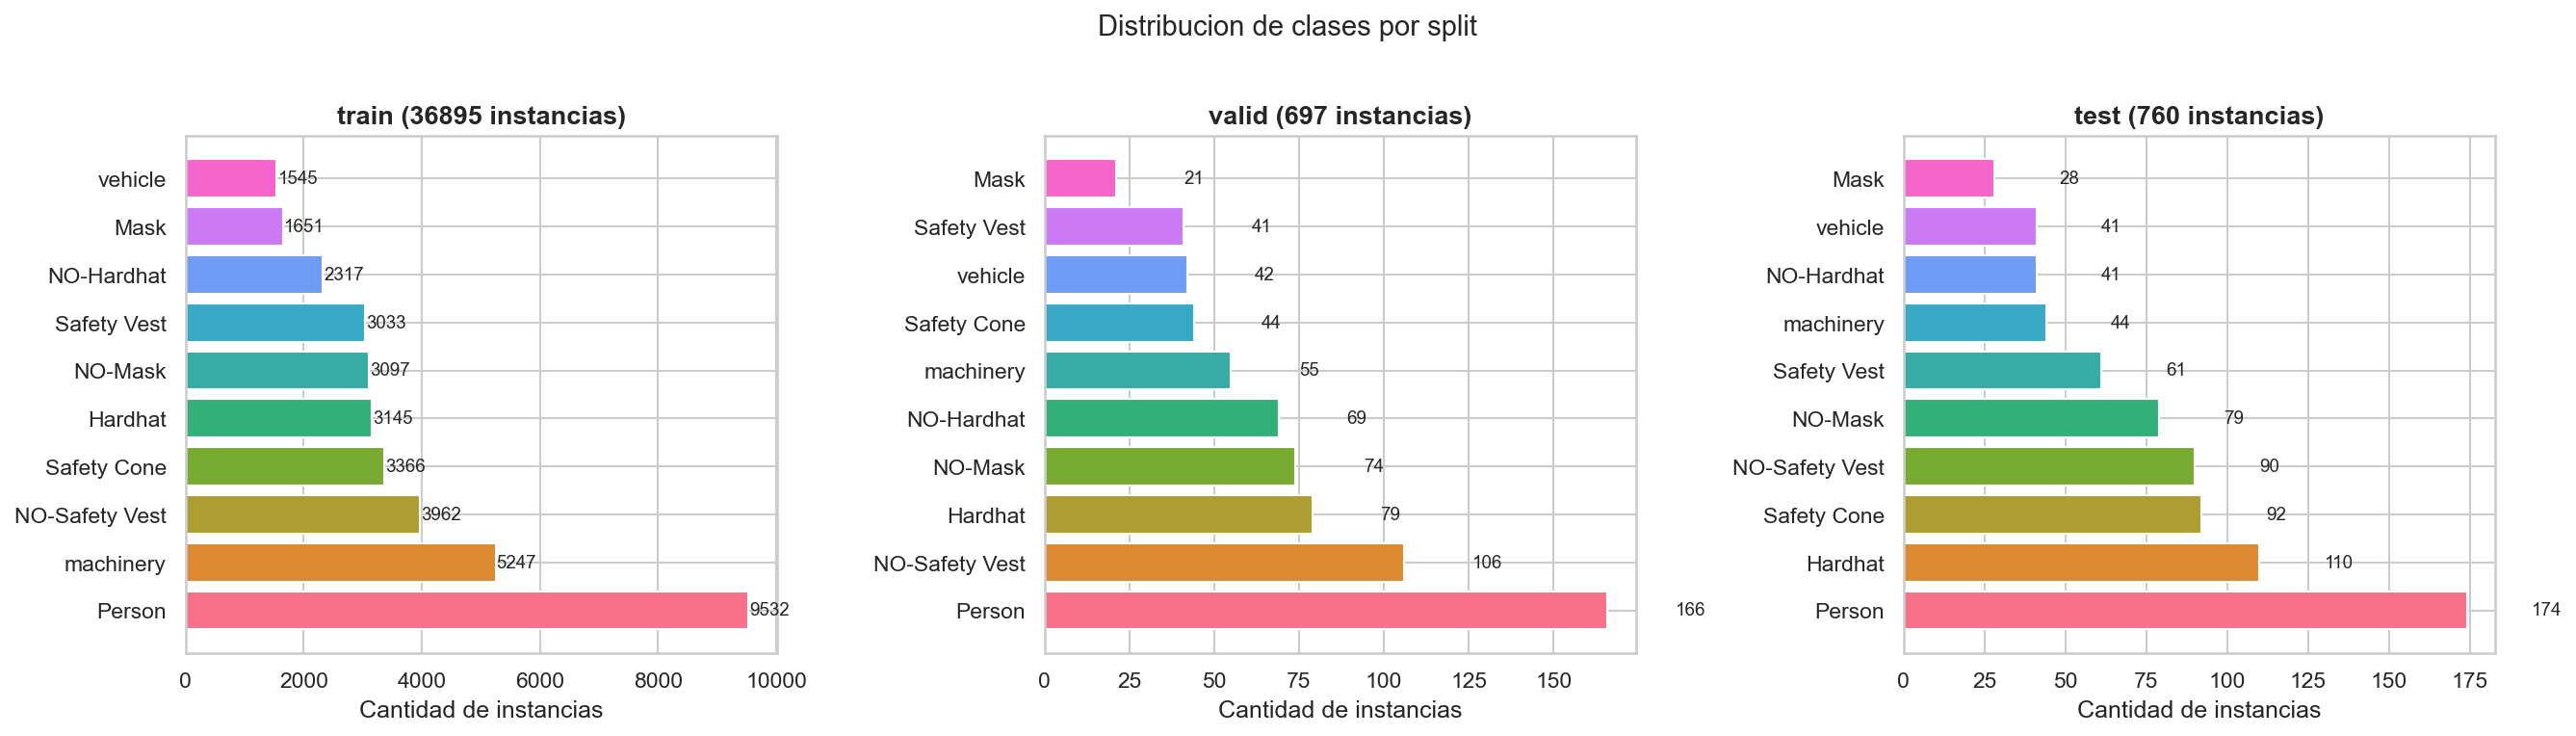
\includegraphics[width=\columnwidth]{class_distribution.png}
    \caption{Distribución de clases por split del dataset.}
    \label{fig:class_dist}
\end{figure}

\subsubsection{Tamaño de Bounding Boxes por Clase}

El análisis de tamaños revela que los elementos de EPP ocupan áreas muy pequeñas en las imágenes (Fig.~\ref{fig:bbox_class}). Hardhat tiene una mediana de área de apenas 0.19\% de la imagen, mientras que Person ocupa 6.2\%. Esta diferencia de escala explica la mayor dificultad del modelo para detectar EPP, especialmente a distancia.

\begin{figure}[h]
    \centering
    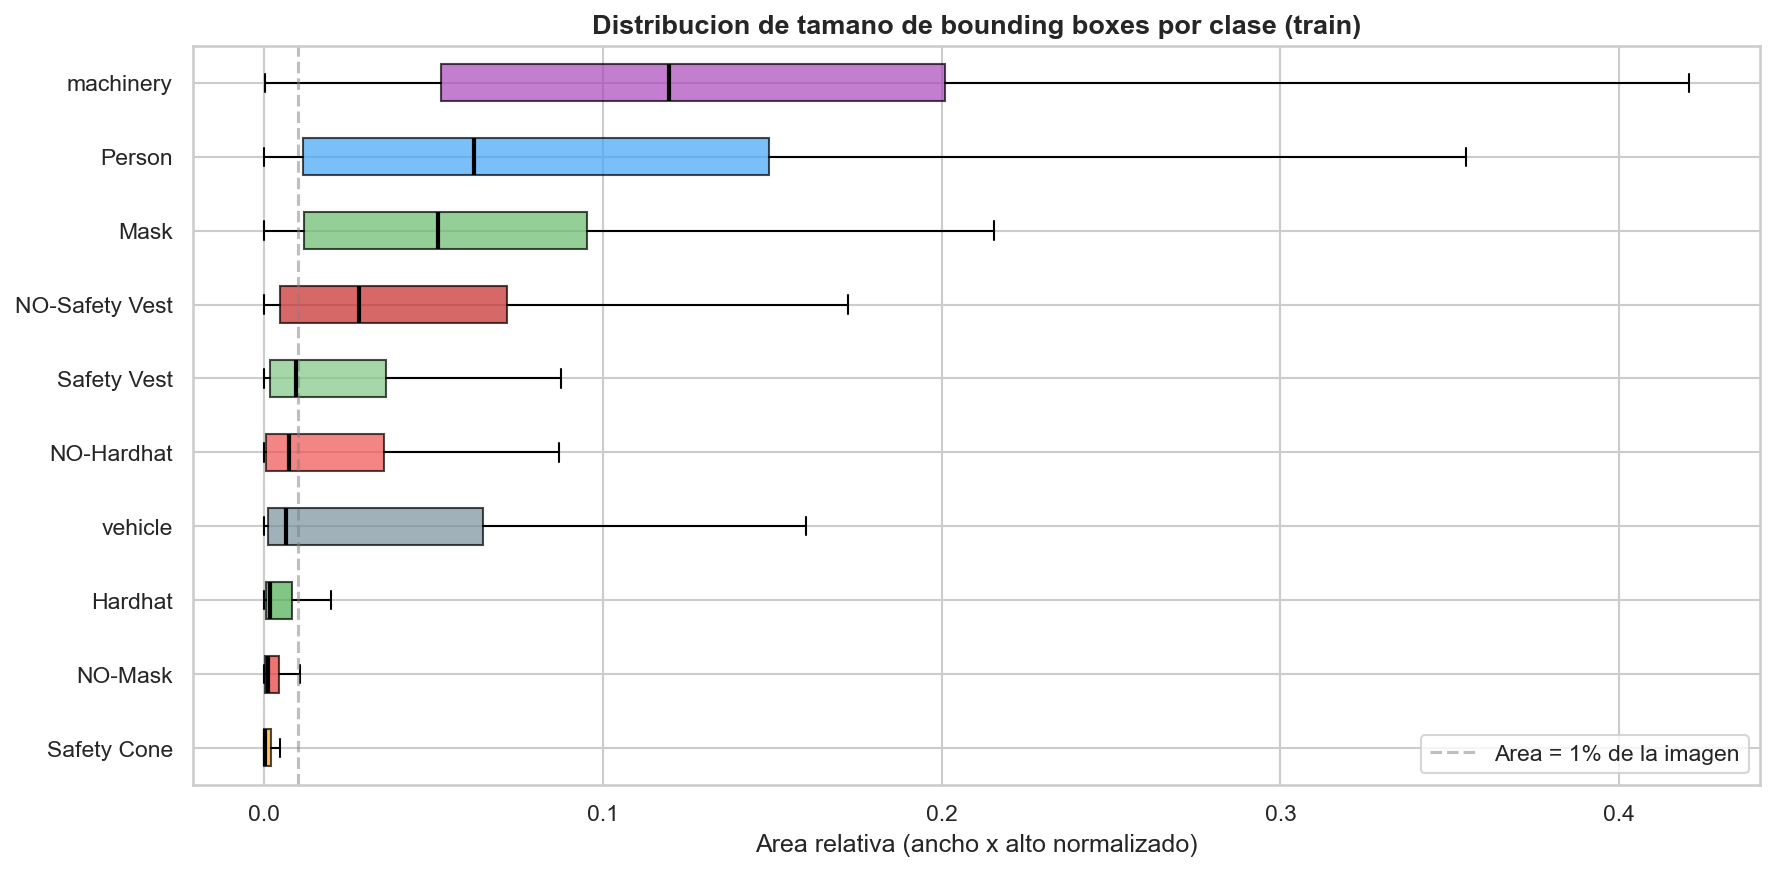
\includegraphics[width=\columnwidth]{bbox_size_per_class.png}
    \caption{Distribución de tamaño de bounding boxes por clase. Los elementos de EPP son significativamente más pequeños que Person o machinery.}
    \label{fig:bbox_class}
\end{figure}

\subsubsection{Co-ocurrencia de Clases}

La matriz de co-ocurrencia normalizada (Fig.~\ref{fig:cooc}) muestra que Hardhat y NO-Hardhat co-ocurren en el 48\% de las imágenes, y Safety Vest y NO-Safety Vest en el 65\%. Esto indica que el dataset contiene escenas mixtas donde conviven trabajadores con y sin EPP, lo cual es valioso para que el modelo aprenda a distinguir ambos casos en un mismo contexto visual. La co-ocurrencia Mask/NO-Mask es más baja (36\%), sugiriendo escenas más homogéneas respecto al uso de barbijo.

\begin{figure}[h]
    \centering
    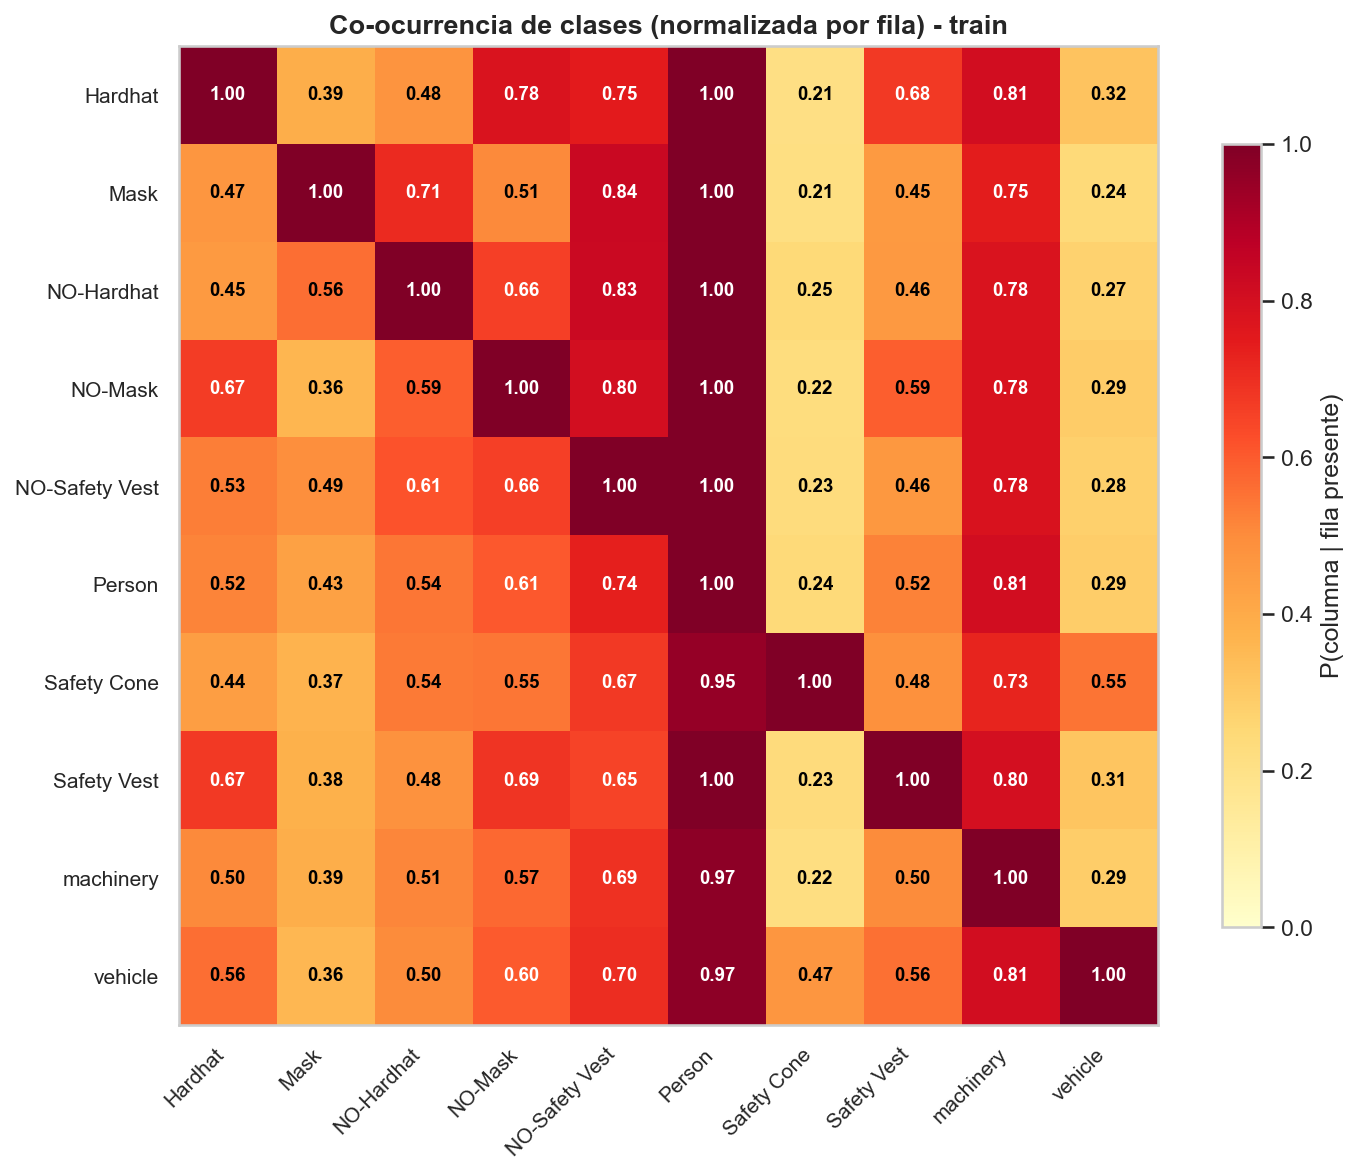
\includegraphics[width=\columnwidth]{class_cooccurrence.png}
    \caption{Co-ocurrencia de clases normalizada por fila.}
    \label{fig:cooc}
\end{figure}

\subsubsection{Densidad de Anotaciones}

Cada imagen contiene en promedio 11 objetos anotados, con una mediana de 3 personas y 5 items de EPP por imagen. Las escenas con alta densidad de trabajadores representan un desafío adicional por las oclusiones parciales y la necesidad de asociar correctamente cada EPP a su persona correspondiente.

% ============================================================
\section{Metodología}

\subsection{Arquitectura del Sistema}

El sistema propuesto sigue un pipeline de cuatro etapas (Fig.~\ref{fig:arch}):

\begin{enumerate}
    \item \textbf{Detección:} Un modelo YOLO fine-tuneado detecta personas, EPP presente y EPP ausente en cada frame.
    \item \textbf{Asociación espacial:} Se asocian las detecciones de EPP a personas mediante overlap de bounding boxes (IoU de contención $>$ 0.3).
    \item \textbf{Tracking:} ByteTrack asigna un Track ID persistente a cada persona a lo largo del video.
    \item \textbf{Compliance:} Un motor de evaluación con ventana deslizante determina el estado de cumplimiento de cada trabajador.
\end{enumerate}

\begin{figure}[h]
    \centering
    \fbox{\parbox{0.9\columnwidth}{\centering
    \texttt{Video} $\rightarrow$ \texttt{YOLO} $\rightarrow$ \texttt{Asociación EPP-Persona} \\
    $\rightarrow$ \texttt{ByteTrack} $\rightarrow$ \texttt{Motor Compliance} $\rightarrow$ \texttt{Alertas}
    }}
    \caption{Pipeline del sistema de monitoreo de EPP.}
    \label{fig:arch}
\end{figure}

\subsection{Fine-tuning de Modelos YOLO}

Se entrenaron tres variantes de YOLO sobre el dataset Construction Site Safety:

\begin{itemize}
    \item \textbf{YOLOv8n} (nano): 3.2M parámetros, optimizado para velocidad.
    \item \textbf{YOLOv8m} (medium): 25.9M parámetros, balance entre precisión y velocidad.
    \item \textbf{YOLOv11n} (nano): arquitectura más reciente con optimizaciones de eficiencia.
\end{itemize}

El entrenamiento se realizó con transfer learning desde pesos pre-entrenados en COCO, utilizando una resolución de entrada de 640$\times$640 píxeles.

\subsection{Motor de Compliance con Tres Estados}

Una contribución clave del sistema es el motor de compliance que evalúa \textbf{cada EPP de forma independiente}, distinguiendo tres estados por frame para cada elemento requerido:

\begin{table}[h]
\centering
\caption{Sistema de tres estados para evaluación de EPP}
\label{tab:tres_estados}
\begin{tabular}{@{}lll@{}}
\toprule
\textbf{Detección} & \textbf{Estado} & \textbf{Significado} \\
\midrule
Detectó EPP presente & CUMPLE & Tiene el EPP \\
Detectó NO-X & NO\_CUMPLE & Confirmado sin EPP \\
No detectó nada & SIN\_DATO & Modelo no pudo decidir \\
\bottomrule
\end{tabular}
\end{table}

La evaluación temporal se realiza con una ventana deslizante de $W$ frames \textbf{por EPP por trabajador}. Cada elemento de protección tiene su propio historial independiente, lo que evita que la falta de detección de un EPP afecte la evaluación de otro. Para cada par (trabajador, EPP), se calcula el ratio de frames SIN\_DATO ($r_{sd}$) en la ventana:

\begin{itemize}
    \item Si $r_{sd} < 0.4$: suficientes datos. Se calcula compliance solo con frames decisivos: $C = \frac{N_{cumple}}{N_{cumple} + N_{no\_cumple}}$. Si $C < 0.3$, se genera alerta.
    \item Si $0.4 \leq r_{sd} \leq 0.7$: datos insuficientes. Estado \textit{indeterminado}.
    \item Si $r_{sd} > 0.7$: el modelo casi nunca detecta EPP en este trabajador. Se asume \textit{no cumple}.
\end{itemize}

Esta lógica, aplicada de forma granular por EPP, evita penalizar a trabajadores cuando el modelo simplemente no logra detectar un elemento específico (por distancia, oclusión o ángulo desfavorable), pero al mismo tiempo marca como incumplidores a aquellos cuyo EPP nunca es visible. La evaluación independiente es crucial porque en un mismo frame el modelo puede detectar correctamente el chaleco pero no el casco (por ejemplo, si el casco está ocluido por el ángulo): con evaluación por frame, ambos EPP recibirían el mismo estado, mientras que con evaluación por EPP, el chaleco recibe CUMPLE y el casco recibe SIN\_DATO.

% ============================================================
\section{Resultados Experimentales}

\subsection{Comparación de Modelos}

La Tabla~\ref{tab:modelos} resume las métricas de evaluación de los tres modelos entrenados.

\begin{table}[h]
\centering
\caption{Comparación de modelos sobre el set de validación}
\label{tab:modelos}
\begin{tabular}{@{}lcccc@{}}
\toprule
\textbf{Modelo} & \textbf{mAP50} & \textbf{mAP50-95} & \textbf{Precision} & \textbf{Recall} \\
\midrule
YOLOv8n  & 0.777 & 0.476 & 0.896 & 0.685 \\
YOLOv8m  & \textbf{0.858} & \textbf{0.580} & \textbf{0.936} & \textbf{0.787} \\
YOLOv11n & 0.769 & 0.461 & 0.888 & 0.698 \\
\bottomrule
\end{tabular}
\end{table}

YOLOv8m obtiene los mejores resultados en todas las métricas, con un mAP50 de 85.8\% y un recall de 78.7\%. En cuanto a velocidad de inferencia (Tabla~\ref{tab:latencia}), los tres modelos operan por encima de 97 FPS en CPU (Apple M3 Max), siendo viables para aplicaciones en tiempo real.

\begin{table}[h]
\centering
\caption{Latencia de inferencia (CPU, Apple M3 Max)}
\label{tab:latencia}
\begin{tabular}{@{}lccc@{}}
\toprule
\textbf{Modelo} & \textbf{Media (ms)} & \textbf{P95 (ms)} & \textbf{FPS} \\
\midrule
YOLOv8n  & 8.3  & 8.5  & 119.9 \\
YOLOv8m  & 10.3 & 10.5 & 97.4  \\
YOLOv11n & 10.3 & 10.7 & 97.2  \\
\bottomrule
\end{tabular}
\end{table}

\subsection{Análisis de la Matriz de Confusión}

La matriz de confusión normalizada del mejor modelo (YOLOv8m, Fig.~\ref{fig:confusion}) revela patrones relevantes para el sistema de compliance:

\begin{figure}[h]
    \centering
    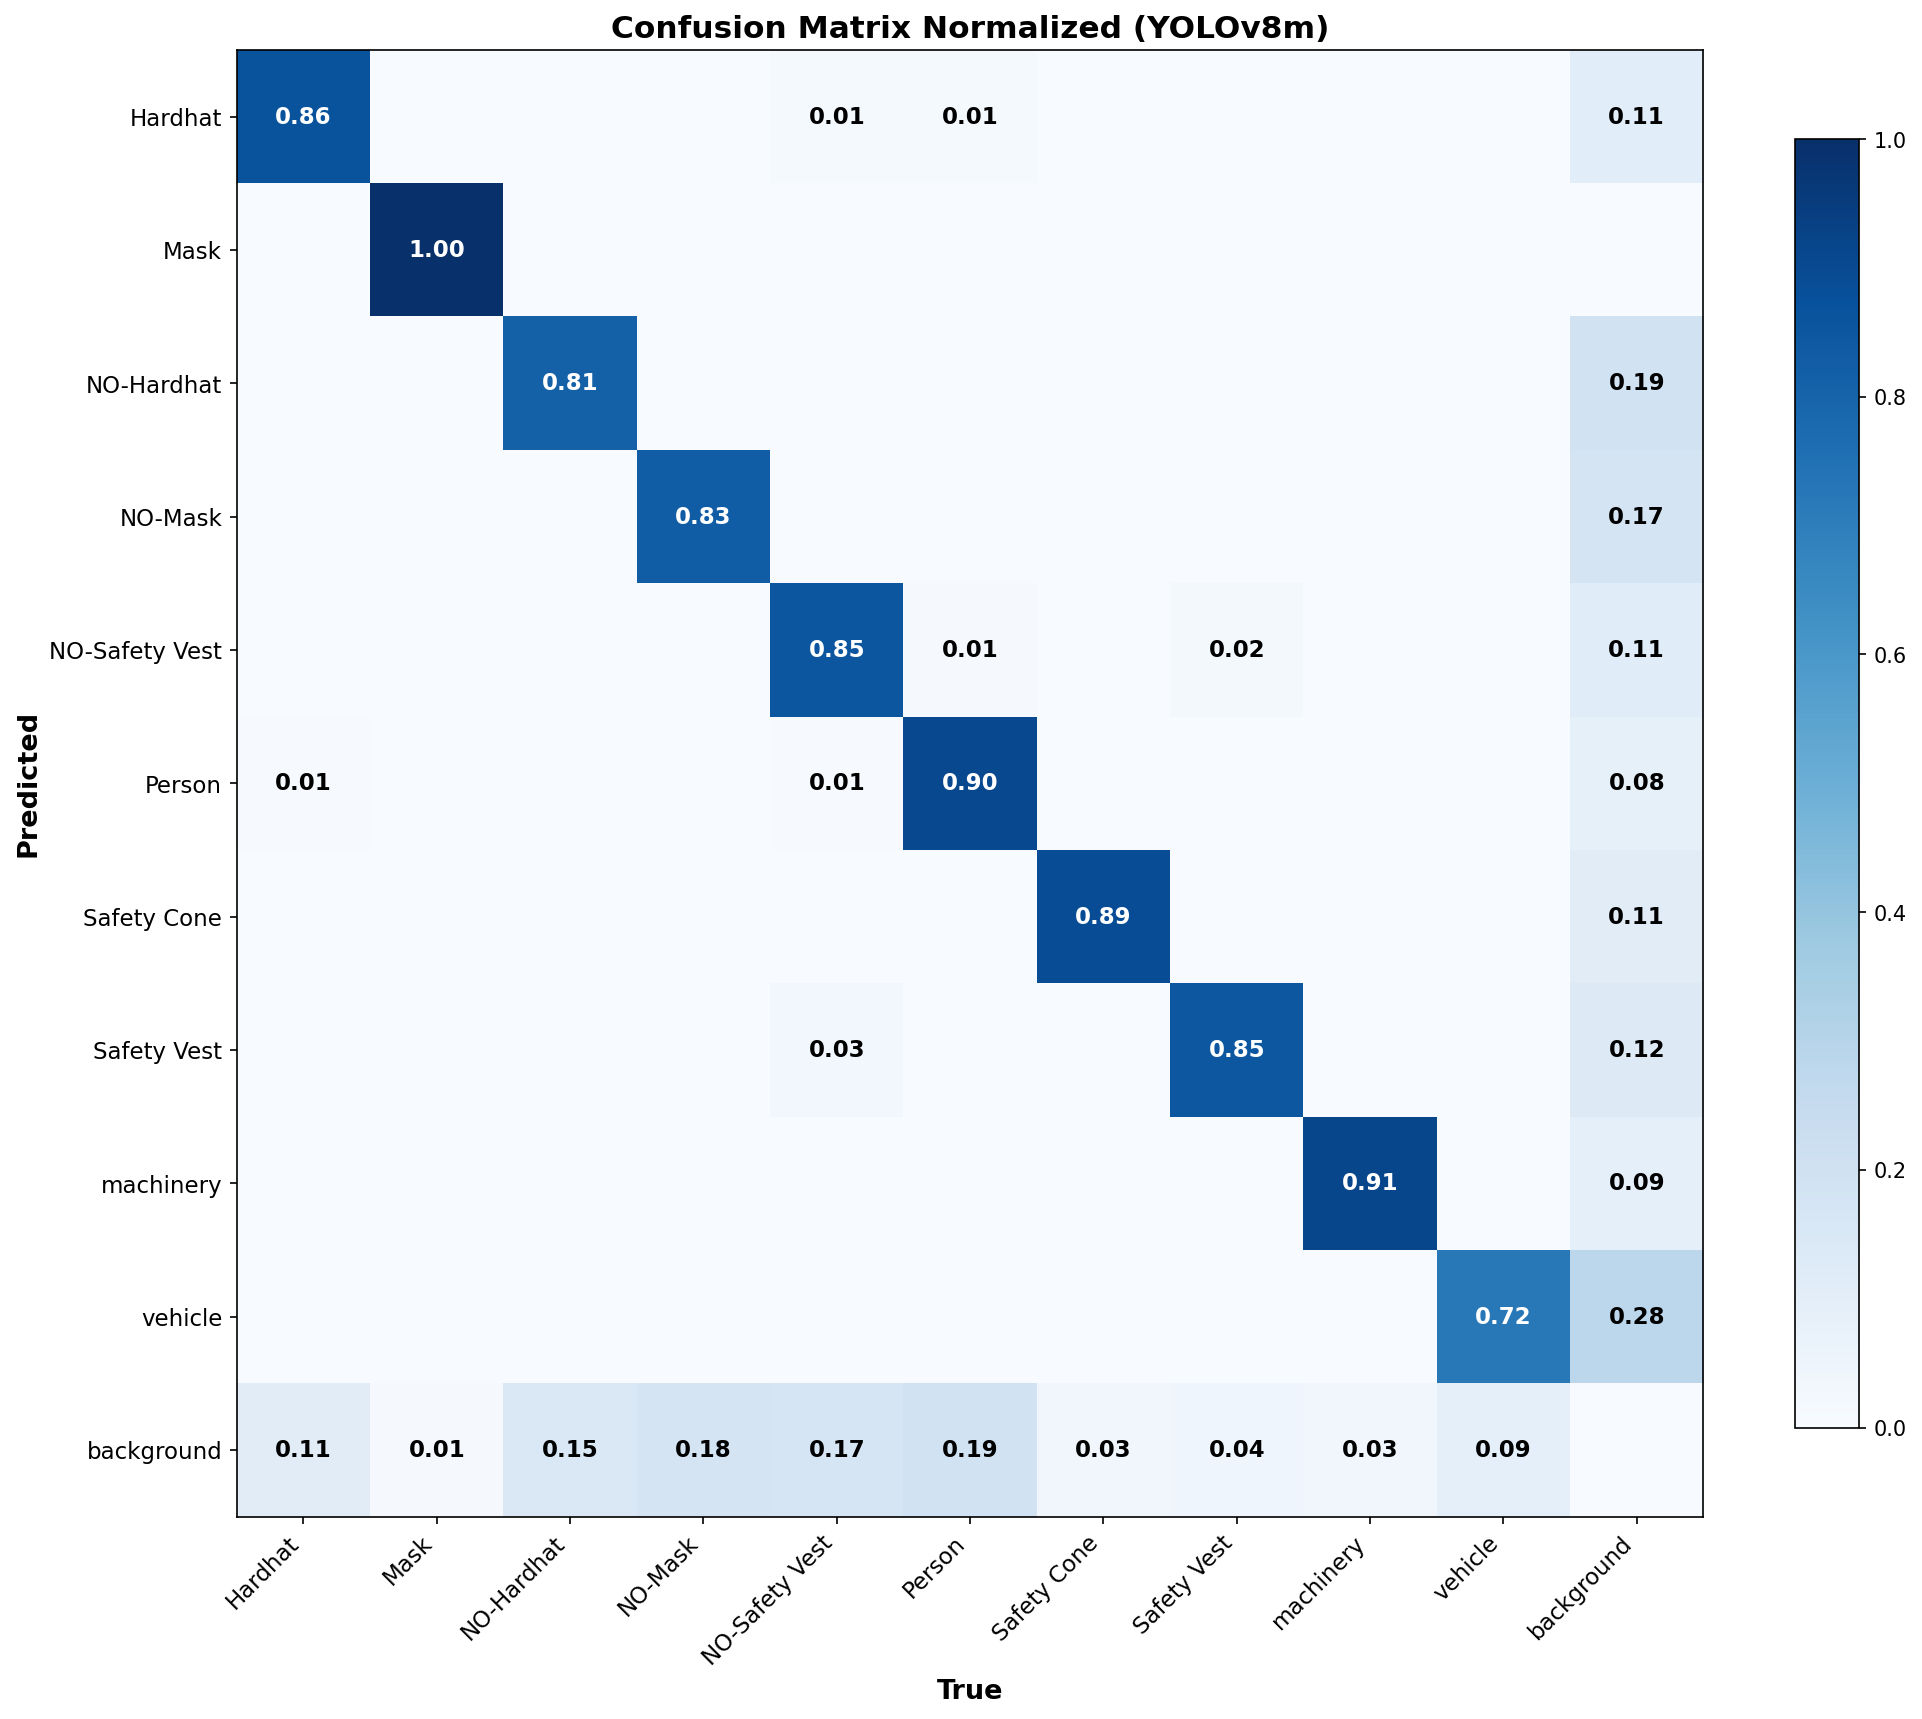
\includegraphics[width=\columnwidth]{confusion_matrix_clean.png}
    \caption{Matriz de confusión normalizada del modelo YOLOv8m.}
    \label{fig:confusion}
\end{figure}

\begin{itemize}
    \item Mask alcanza 100\% de accuracy, beneficiada por bounding boxes relativamente grandes (mediana de área 5.1\%).
    \item Person y machinery superan el 90\%, siendo objetos grandes y visualmente distintivos.
    \item Las clases NO-X obtienen entre 81--85\% de accuracy, con pérdidas del 11--19\% hacia background. Detectar la \textit{ausencia} de un objeto es inherentemente más difícil.
    \item Hardhat alcanza 86\%, con 11\% perdido a background. Al ser el EPP más pequeño (mediana 0.19\% del área), es esperable mayor dificultad.
    \item vehicle es la clase con menor accuracy (72\%), con 28\% de pérdida a background.
\end{itemize}

La pérdida hacia background de las clases NO-X (11--19\%) justifica directamente la implementación del sistema de tres estados: en esos frames donde el modelo no detecta ni presencia ni ausencia, el estado SIN\_DATO evita generar falsos positivos de compliance o falsas alertas de incumplimiento.

\subsection{Evaluación del Sistema de Tracking y Compliance}

El sistema fue evaluado sobre cinco videos reales de obras de construcción, monitoreando Hardhat y Safety Vest como EPP requeridos (Tabla~\ref{tab:demo}).

\begin{table}[h]
\centering
\caption{Resultados del sistema sobre videos de prueba}
\label{tab:demo}
\begin{tabular}{@{}lcccc@{}}
\toprule
\textbf{Video} & \textbf{Frames} & \textbf{Tracks} & \textbf{Alertas} & \textbf{Compl.} \\
\midrule
Vista general     & 607 & 49 & 78 & 63.1\% \\
Con maquinaria    & 456 & 10 & 8  & 42.4\%  \\
Aire libre        & 447 & 10 & 8  & 53.6\%  \\
Colaboración      & 235 & 8  & 8  & 74.5\% \\
EPP completo      & 201 & 5  & 3  & 100.0\% \\
\bottomrule
\end{tabular}
\end{table}

El video ``EPP completo'', donde todos los trabajadores portan el equipamiento de seguridad, obtiene un compliance de 100\%, validando la efectividad de la evaluación por EPP individual con tres estados. Antes de implementar esta lógica, el mismo video obtenía solo 61\% de compliance porque frames donde el modelo no detectaba uno de los dos EPP (por ejemplo, el casco ocluido por el ángulo) penalizaban la evaluación de ambos elementos simultáneamente. Con la evaluación independiente por EPP, cada elemento tiene su propio historial y los frames SIN\_DATO de un EPP no afectan al otro.

% ============================================================
\section{Discusión}

\subsection{Limitaciones del Detector}

La principal limitación del sistema proviene del recall de las clases NO-X (81--85\%). El modelo pierde entre 11 y 19\% de las detecciones de ausencia de EPP, clasificándolas como background. Este comportamiento se explica por dos factores:

\begin{enumerate}
    \item \textbf{Tamaño reducido de los objetos:} los EPP ocupan menos del 2\% del área de la imagen en la mayoría de los casos, lo que dificulta la detección a distancia.
    \item \textbf{Dificultad intrínseca de detectar ausencia:} las clases NO-X no representan un objeto físico sino la ausencia de uno, lo que implica mayor variabilidad visual y menor cantidad de features discriminativas.
\end{enumerate}

\subsection{Efectividad de la Evaluación por EPP Individual}

La combinación de tres estados con evaluación independiente por EPP produce mejoras significativas en la precisión del compliance. El caso más ilustrativo es el video ``EPP completo'': con evaluación a nivel de frame, el compliance era de 61\% a pesar de que todos los trabajadores tenían casco y chaleco, porque en frames donde el modelo detectaba el chaleco pero no el casco, todo el frame se marcaba como SIN\_DATO o NO\_CUMPLE para ambos EPP. Con la evaluación individual, el compliance alcanza el 100\% esperado.

Los umbrales de ratio de SIN\_DATO (0.4 y 0.7) permiten manejar de forma graduada los escenarios donde:

\begin{itemize}
    \item Los trabajadores están lejos de la cámara y los EPP son difíciles de resolver.
    \item Hay oclusiones parciales que impiden la detección momentánea de un EPP específico.
    \item El ángulo de la cámara no favorece la visibilidad de ciertos elementos.
\end{itemize}

\subsection{Consideraciones para Despliegue}

Para un sistema productivo, se recomienda:
\begin{itemize}
    \item Utilizar múltiples cámaras con diferentes ángulos para maximizar la cobertura.
    \item Emplear modelos de mayor capacidad (YOLOv8l o YOLOv8x) con aceleración GPU para mejorar el recall en las clases NO-X.
    \item Ajustar los umbrales del motor de compliance según el nivel de riesgo de cada zona de la obra.
\end{itemize}

% ============================================================
\section{Conclusiones}

Se desarrolló un sistema de monitoreo automático de EPP que integra detección con YOLO, tracking con ByteTrack y un motor de compliance con lógica de tres estados. El sistema es capaz de:

\begin{itemize}
    \item Detectar cascos, chalecos y mascarillas con un mAP50 de 85.8\%.
    \item Asignar identidades persistentes a trabajadores mediante tracking.
    \item Evaluar el cumplimiento de EPP de forma temporal, distinguiendo entre ausencia confirmada y falta de detección.
    \item Generar alertas en tiempo real para trabajadores con incumplimiento persistente.
\end{itemize}

El análisis exploratorio del dataset reveló que los elementos de EPP representan menos del 2\% del área de la imagen, lo que constituye el principal desafío para la detección. El sistema de tres estados propuesto aborda esta limitación de forma robusta, evitando penalizar a trabajadores cuando el detector falla por distancia u oclusión.

Como trabajo futuro, se plantea: (1) implementar perfiles de monitoreo configurables por zona de obra, permitiendo definir qué EPP es requerido según el tipo de actividad o área (por ejemplo, exigir mascarilla solo en zonas de corte o soldadura, mientras que en exteriores solo se requieran casco y chaleco); (2) evaluar el impacto de técnicas de data augmentation específicas para objetos pequeños; (3) explorar arquitecturas con módulos de atención espacial para mejorar la detección de las clases NO-X; y (4) validar el sistema en entornos de producción con cámaras de vigilancia reales.

% ============================================================
\begin{thebibliography}{99}

\bibitem{oit2023}
Organización Internacional del Trabajo, ``Safety and Health at Work,'' \textit{ILO Global Estimates}, 2023.

\bibitem{redmon2016yolo}
J. Redmon, S. Divvala, R. Girshick, and A. Farhadi, ``You Only Look Once: Unified, Real-Time Object Detection,'' in \textit{Proc. IEEE CVPR}, 2016, pp. 779--788.

\bibitem{ren2015faster}
S. Ren, K. He, R. Girshick, and J. Sun, ``Faster R-CNN: Towards Real-Time Object Detection with Region Proposal Networks,'' in \textit{Proc. NeurIPS}, 2015.

\bibitem{jocher2023yolov8}
G. Jocher, A. Chaurasia, and J. Qiu, ``Ultralytics YOLOv8,'' 2023. [Online]. Available: \url{https://github.com/ultralytics/ultralytics}

\bibitem{jocher2024yolov11}
G. Jocher and J. Qiu, ``Ultralytics YOLO11,'' 2024. [Online]. Available: \url{https://docs.ultralytics.com/models/yolo11/}

\bibitem{bewley2016sort}
A. Bewley, Z. Ge, L. Ott, F. Ramos, and B. Upcroft, ``Simple Online and Realtime Tracking,'' in \textit{Proc. IEEE ICIP}, 2016, pp. 3464--3468.

\bibitem{wojke2017deep}
N. Wojke, A. Bewley, and D. Paulus, ``Simple Online and Realtime Tracking with a Deep Association Metric,'' in \textit{Proc. IEEE ICIP}, 2017.

\bibitem{zhang2022bytetrack}
Y. Zhang, P. Sun, Y. Jiang, et al., ``ByteTrack: Multi-Object Tracking by Associating Every Detection Box,'' in \textit{Proc. ECCV}, 2022, pp. 1--21.

\bibitem{nath2020deep}
N. D. Nath, A. H. Behzadan, and S. G. Paal, ``Deep learning for site safety: Real-time detection of personal protective equipment,'' \textit{Automation in Construction}, vol. 112, 2020.

\bibitem{delhi2020detection}
V. S. K. Delhi, R. Sankarlal, and A. Thomas, ``Detection of Personal Protective Equipment (PPE) Compliance on Construction Site Using Computer Vision Based Deep Learning Techniques,'' \textit{Frontiers in Built Environment}, vol. 6, 2020.

\bibitem{wang2021ppe}
Z. Wang, Y. Wu, Q. Yang, and F. Li, ``Construction workers' personal protective equipment detection based on improved YOLOv5,'' \textit{Applied Sciences}, vol. 11, no. 15, 2021.

\end{thebibliography}

\end{document}
